\subsection{Hauptoberfläche}

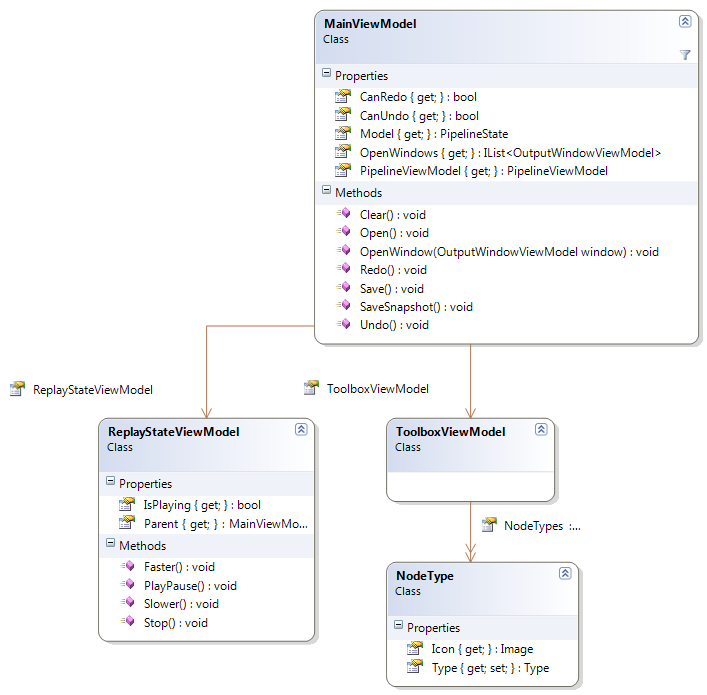
\includegraphics[width=\textwidth]{YuvKA.ViewModel/main.png}
Das Programm wird durch Instanziierung des \name{MainViewModel}s und Anzeigen der zugehörigen View gestartet. Diese Klasse delegiert Einheiten der Hauptoberfläche an untergeordnete View Models, wobei die Klassen zur Anzeige des Pipeline-Graphen in einem eigenen Abschnitt beschrieben werden.

\subsubsection{MainViewModel}

\begin{verbatim}
public class MainViewModel
\end{verbatim}

\paragraph{Beschreibung}~\\
Die \name{MainViewModel}-Klasse hält das Programm-Model in Form einer \name{PipelineState}-Instanz, verwaltet es in einem Undo/Redo-System und instanziiert weitere untergeordnete View Models.

\paragraph{Typmember}
\begin{itemize}

\property{CanUndo, CanRedo}
	\begin{verbatim}
	public bool CanUndo { get; }
	public bool CanRedo { get; }
	\end{verbatim}
	Ruft ab, ob ein Rückgängig- bzw. Wiederholen-Schritt zur Verfügung steht.

\property{Model}
	\INPC
	\begin{verbatim}
	public PipelineState Model { get; }
	\end{verbatim}
	Stellt das derzeitige Model-Objekt für Data Binding und untergeordnete View Models zur Verfügung.

\property{OpenWindows}
	\begin{verbatim}
	public IList<OutputWindowViewModel> OpenWindows { get; }
	\end{verbatim}
	Ruft eine Liste der derzeit geöffneten Ausgabefenster ab.

\property{ReplayStateViewModel, PipelineViewModel, ToolboxViewModel}

	Rufen jeweils eine Instanz der gleichnamigen Klasse ab.

\method{Clear, Open}
	\begin{verbatim}
	public void Clear()
	public void Open()
	\end{verbatim}
	Ersetzen das derzeitige Model durch eine neue leere bzw. aus einer Datei geladenen Pipeline, dabei wird jeweils ein neuer Rückgängig-Schritt erzeugt. Open öffnet zusätzlich einen \name{OpenFileDialog} zur Auswahl des Dateipfades.

\method{Save}
	\begin{verbatim}
	public void Save()
	\end{verbatim}
	Speichert das derzeitige Model in einer Datei ab. Dazu öffnet Save einen \name{SaveFileDialog} und serialisiert dann das \name{Model}-Objekt in die gewählte Datei.

\method{SaveSnapshot}
	\begin{verbatim}
	public void SaveSnapshot()
	\end{verbatim}
	Hält den aktuellen Model-Zustand als Rückgängig-Schritt fest. Alle Wiederholen-Schritte werden verworfen.

\method{Undo, Redo}
	\begin{verbatim}
	public void Undo()
	public void Redo()
	\end{verbatim}
	Stellt den Zustand des nächsten Rückgängig- bzw. Wiederholen-Schrittes wieder her.

\end{itemize}

\subsubsection{ReplayStateViewModel}

\begin{verbatim}
public class ReplayStateViewModel
\end{verbatim}

\paragraph{Beschreibung}~\\
Die \name{ReplayStateViewModel}-Klasse verwaltet den aktuellen Wiedergabestatus der geöffneten Pipeline.

\paragraph{Typmember}
\begin{itemize}

\property{IsPlaying}
	\begin{verbatim}
	public bool IsPlaying { get; }
	\end{verbatim}
	Ruft ab, ob die Pipeline gerade abgespielt wird.

\method{Slower, Faster}
	\begin{verbatim}
	public void Slower()
	public void Faster()
	\end{verbatim}
	Erniedrigt bzw. erhöht die Abspielgeschwindigkeit um einen konstanten Faktor, der im Ermessen der Implementierung liegt.

\method{PlayPause}
	\begin{verbatim}
	public void PlayPause()
	\end{verbatim}
	Pausiert die Wiedergabe bzw. setzt sie fort.

\method{Stop}
	\begin{verbatim}
	public void Stop()
	\end{verbatim}
	Pausiert die Wiedergabe und setzt \name{CurrentTick} auf 0.

\end{itemize}

\subsubsection{YuvKA.ViewModel.ToolboxViewModel}

\begin{verbatim}
public class ToolboxViewModel
\end{verbatim}

\paragraph{Beschreibung}~\\
Die \name{ToolboxViewModel}-Klasse ist dafür zuständig, die dynamisch erweiterbare Menge der Knotentypen zu ermitteln.

\paragraph{Typmember}
\begin{itemize}

\property{NodeTypes}
	\begin{verbatim}
	public IList<NodeType> NodeTypes { get; }
	\end{verbatim}
	Ruft die Menge der geladenen Knotentypen ab.

\end{itemize}

\subsubsection{YuvKA.ViewModel.NodeType}

\begin{verbatim}
public class NodeType
\end{verbatim}

\paragraph{Beschreibung}~\\
Die \name{NodeType}-Klasse hält die \name{Type}-Instanz und das Icon eines dynamisch geladenen Knotentyps.

\paragraph{Typmember}
\begin{itemize}

\property{Icon}
	\begin{verbatim}
	public Image Icon { get; }
	\end{verbatim}
	Ruft das Icon des Knotentyps ab, falls verfügbar. Hierzu muss der Knotentyp mit dem \name{ToolboxBitmapAttribute} annotiert sein.

\method{Type}
	\begin{verbatim}
	public Type Type { get; set; }
	\end{verbatim}
	Ruft den CLR-Typ des Knotentyps ab oder legt ihn fest. Über diesen Wert kann der Knotentyp instanziiert werden.

\end{itemize}